
%% bare_conf_compsoc.tex
%% V1.4a
%% 2014/09/17
%% by Michael Shell
%% See:
%% http://www.michaelshell.org/
%% for current contact information.
%%
%% This is a skeleton file demonstrating the use of IEEEtran.cls
%% (requires IEEEtran.cls version 1.8s or later) with an IEEE Computer
%% Society conference paper.
%%
%% Support sites:
%% http://www.michaelshell.org/tex/ieeetran/
%% http://www.ctan.org/tex-archive/macros/latex/contrib/IEEEtran/
%% and
%% http://www.ieee.org/

%%*************************************************************************
%% Legal Notice:
%% This code is offered as-is without any warranty either expressed or
%% implied; without even the implied warranty of MERCHANTABILITY or
%% FITNESS FOR A PARTICULAR PURPOSE! 
%% User assumes all risk.
%% In no event shall IEEE or any contributor to this code be liable for
%% any damages or losses, including, but not limited to, incidental,
%% consequential, or any other damages, resulting from the use or misuse
%% of any information contained here.
%%
%% All comments are the opinions of their respective authors and are not
%% necessarily endorsed by the IEEE.
%%
%% This work is distributed under the LaTeX Project Public License (LPPL)
%% ( http://www.latex-project.org/ ) version 1.3, and may be freely used,
%% distributed and modified. A copy of the LPPL, version 1.3, is included
%% in the base LaTeX documentation of all distributions of LaTeX released
%% 2003/12/01 or later.
%% Retain all contribution notices and credits.
%% ** Modified files should be clearly indicated as such, including  **
%% ** renaming them and changing author support contact information. **
%%
%% File list of work: IEEEtran.cls, IEEEtran_HOWTO.pdf, bare_adv.tex,
%%                    bare_conf.tex, bare_jrnl.tex, bare_conf_compsoc.tex,
%%                    bare_jrnl_compsoc.tex, bare_jrnl_transmag.tex
%%*************************************************************************


% *** Authors should verify (and, if needed, correct) their LaTeX system  ***
% *** with the testflow diagnostic prior to trusting their LaTeX platform ***
% *** with production work. IEEE's font choices and paper sizes can       ***
% *** trigger bugs that do not appear when using other class files.       ***                          ***
% The testflow support page is at:
% http://www.michaelshell.org/tex/testflow/



\documentclass[10pt, conference,compsoc]{IEEEtran}
% Some/most Computer Society conferences require the compsoc mode option,
% but others may want the standard conference format.
%
% If IEEEtran.cls has not been installed into the LaTeX system files,
% manually specify the path to it like:
% \documentclass[conference,compsoc]{../sty/IEEEtran}

\usepackage{listings}



% Some very useful LaTeX packages include:
% (uncomment the ones you want to load)


% *** MISC UTILITY PACKAGES ***
%
%\usepackage{ifpdf}
% Heiko Oberdiek's ifpdf.sty is very useful if you need conditional
% compilation based on whether the output is pdf or dvi.
% usage:
% \ifpdf
%   % pdf code
% \else
%   % dvi code
% \fi
% The latest version of ifpdf.sty can be obtained from:
% http://www.ctan.org/tex-archive/macros/latex/contrib/oberdiek/
% Also, note that IEEEtran.cls V1.7 and later provides a builtin
% \ifCLASSINFOpdf conditional that works the same way.
% When switching from latex to pdflatex and vice-versa, the compiler may
% have to be run twice to clear warning/error messages.






% *** CITATION PACKAGES ***
%
\ifCLASSOPTIONcompsoc
  % IEEE Computer Society needs nocompress option
  % requires cite.sty v4.0 or later (November 2003)
  \usepackage[nocompress]{cite}
\else
  % normal IEEE
  \usepackage{cite}
\fi
% cite.sty was written by Donald Arseneau
% V1.6 and later of IEEEtran pre-defines the format of the cite.sty package
% \cite{} output to follow that of IEEE. Loading the cite package will
% result in citation numbers being automatically sorted and properly
% "compressed/ranged". e.g., [1], [9], [2], [7], [5], [6] without using
% cite.sty will become [1], [2], [5]--[7], [9] using cite.sty. cite.sty's
% \cite will automatically add leading space, if needed. Use cite.sty's
% noadjust option (cite.sty V3.8 and later) if you want to turn this off
% such as if a citation ever needs to be enclosed in parenthesis.
% cite.sty is already installed on most LaTeX systems. Be sure and use
% version 5.0 (2009-03-20) and later if using hyperref.sty.
% The latest version can be obtained at:
% http://www.ctan.org/tex-archive/macros/latex/contrib/cite/
% The documentation is contained in the cite.sty file itself.
%
% Note that some packages require special options to format as the Computer
% Society requires. In particular, Computer Society  papers do not use
% compressed citation ranges as is done in typical IEEE papers
% (e.g., [1]-[4]). Instead, they list every citation separately in order
% (e.g., [1], [2], [3], [4]). To get the latter we need to load the cite
% package with the nocompress option which is supported by cite.sty v4.0
% and later.





% *** GRAPHICS RELATED PACKAGES ***
%
\ifCLASSINFOpdf
  \usepackage[pdftex]{graphicx}
  % declare the path(s) where your graphic files are
  % \graphicspath{{../pdf/}{../jpeg/}}
  % and their extensions so you won't have to specify these with
  % every instance of \includegraphics
  % \DeclareGraphicsExtensions{.pdf,.jpeg,.png}
\else
  % or other class option (dvipsone, dvipdf, if not using dvips). graphicx
  % will default to the driver specified in the system graphics.cfg if no
  % driver is specified.
  % \usepackage[dvips]{graphicx}
  % declare the path(s) where your graphic files are
  % \graphicspath{{../eps/}}
  % and their extensions so you won't have to specify these with
  % every instance of \includegraphics
  % \DeclareGraphicsExtensions{.eps}
\fi
% graphicx was written by David Carlisle and Sebastian Rahtz. It is
% required if you want graphics, photos, etc. graphicx.sty is already
% installed on most LaTeX systems. The latest version and documentation
% can be obtained at: 
% http://www.ctan.org/tex-archive/macros/latex/required/graphics/
% Another good source of documentation is "Using Imported Graphics in
% LaTeX2e" by Keith Reckdahl which can be found at:
% http://www.ctan.org/tex-archive/info/epslatex/
%
% latex, and pdflatex in dvi mode, support graphics in encapsulated
% postscript (.eps) format. pdflatex in pdf mode supports graphics
% in .pdf, .jpeg, .png and .mps (metapost) formats. Users should ensure
% that all non-photo figures use a vector format (.eps, .pdf, .mps) and
% not a bitmapped formats (.jpeg, .png). IEEE frowns on bitmapped formats
% which can result in "jaggedy"/blurry rendering of lines and letters as
% well as large increases in file sizes.
%
% You can find documentation about the pdfTeX application at:
% http://www.tug.org/applications/pdftex





% *** MATH PACKAGES ***
%
\usepackage[cmex10]{amsmath}
% A popular package from the American Mathematical Society that provides
% many useful and powerful commands for dealing with mathematics. If using
% it, be sure to load this package with the cmex10 option to ensure that
% only type 1 fonts will utilized at all point sizes. Without this option,
% it is possible that some math symbols, particularly those within
% footnotes, will be rendered in bitmap form which will result in a
% document that can not be IEEE Xplore compliant!
%
% Also, note that the amsmath package sets \interdisplaylinepenalty to 10000
% thus preventing page breaks from occurring within multiline equations. Use:
%\interdisplaylinepenalty=2500
% after loading amsmath to restore such page breaks as IEEEtran.cls normally
% does. amsmath.sty is already installed on most LaTeX systems. The latest
% version and documentation can be obtained at:
% http://www.ctan.org/tex-archive/macros/latex/required/amslatex/math/





% *** SPECIALIZED LIST PACKAGES ***
%
%\usepackage{algorithmic}
% algorithmic.sty was written by Peter Williams and Rogerio Brito.
% This package provides an algorithmic environment fo describing algorithms.
% You can use the algorithmic environment in-text or within a figure
% environment to provide for a floating algorithm. Do NOT use the algorithm
% floating environment provided by algorithm.sty (by the same authors) or
% algorithm2e.sty (by Christophe Fiorio) as IEEE does not use dedicated
% algorithm float types and packages that provide these will not provide
% correct IEEE style captions. The latest version and documentation of
% algorithmic.sty can be obtained at:
% http://www.ctan.org/tex-archive/macros/latex/contrib/algorithms/
% There is also a support site at:
% http://algorithms.berlios.de/index.html
% Also of interest may be the (relatively newer and more customizable)
% algorithmicx.sty package by Szasz Janos:
% http://www.ctan.org/tex-archive/macros/latex/contrib/algorithmicx/




% *** ALIGNMENT PACKAGES ***
%
%\usepackage{array}
% Frank Mittelbach's and David Carlisle's array.sty patches and improves
% the standard LaTeX2e array and tabular environments to provide better
% appearance and additional user controls. As the default LaTeX2e table
% generation code is lacking to the point of almost being broken with
% respect to the quality of the end results, all users are strongly
% advised to use an enhanced (at the very least that provided by array.sty)
% set of table tools. array.sty is already installed on most systems. The
% latest version and documentation can be obtained at:
% http://www.ctan.org/tex-archive/macros/latex/required/tools/


% IEEEtran contains the IEEEeqnarray family of commands that can be used to
% generate multiline equations as well as matrices, tables, etc., of high
% quality.




% *** SUBFIGURE PACKAGES ***
\ifCLASSOPTIONcompsoc
  \usepackage[caption=false,font=footnotesize,labelfont=sf,textfont=sf]{subfig}
\else
  \usepackage[caption=false,font=footnotesize]{subfig}
\fi
% subfig.sty, written by Steven Douglas Cochran, is the modern replacement
% for subfigure.sty, the latter of which is no longer maintained and is
% incompatible with some LaTeX packages including fixltx2e. However,
% subfig.sty requires and automatically loads Axel Sommerfeldt's caption.sty
% which will override IEEEtran.cls' handling of captions and this will result
% in non-IEEE style figure/table captions. To prevent this problem, be sure
% and invoke subfig.sty's "caption=false" package option (available since
% subfig.sty version 1.3, 2005/06/28) as this is will preserve IEEEtran.cls
% handling of captions.
% Note that the Computer Society format requires a sans serif font rather
% than the serif font used in traditional IEEE formatting and thus the need
% to invoke different subfig.sty package options depending on whether
% compsoc mode has been enabled.
%
% The latest version and documentation of subfig.sty can be obtained at:
% http://www.ctan.org/tex-archive/macros/latex/contrib/subfig/




% *** FLOAT PACKAGES ***
%
%\usepackage{fixltx2e}
% fixltx2e, the successor to the earlier fix2col.sty, was written by
% Frank Mittelbach and David Carlisle. This package corrects a few problems
% in the LaTeX2e kernel, the most notable of which is that in current
% LaTeX2e releases, the ordering of single and double column floats is not
% guaranteed to be preserved. Thus, an unpatched LaTeX2e can allow a
% single column figure to be placed prior to an earlier double column
% figure. The latest version and documentation can be found at:
% http://www.ctan.org/tex-archive/macros/latex/base/


%\usepackage{stfloats}
% stfloats.sty was written by Sigitas Tolusis. This package gives LaTeX2e
% the ability to do double column floats at the bottom of the page as well
% as the top. (e.g., "\begin{figure*}[!b]" is not normally possible in
% LaTeX2e). It also provides a command:
%\fnbelowfloat
% to enable the placement of footnotes below bottom floats (the standard
% LaTeX2e kernel puts them above bottom floats). This is an invasive package
% which rewrites many portions of the LaTeX2e float routines. It may not work
% with other packages that modify the LaTeX2e float routines. The latest
% version and documentation can be obtained at:
% http://www.ctan.org/tex-archive/macros/latex/contrib/sttools/
% Do not use the stfloats baselinefloat ability as IEEE does not allow
% \baselineskip to stretch. Authors submitting work to the IEEE should note
% that IEEE rarely uses double column equations and that authors should try
% to avoid such use. Do not be tempted to use the cuted.sty or midfloat.sty
% packages (also by Sigitas Tolusis) as IEEE does not format its papers in
% such ways.
% Do not attempt to use stfloats with fixltx2e as they are incompatible.
% Instead, use Morten Hogholm'a dblfloatfix which combines the features
% of both fixltx2e and stfloats:
%
% \usepackage{dblfloatfix}
% The latest version can be found at:
% http://www.ctan.org/tex-archive/macros/latex/contrib/dblfloatfix/




% *** PDF, URL AND HYPERLINK PACKAGES ***
%
%\usepackage{url}
% url.sty was written by Donald Arseneau. It provides better support for
% handling and breaking URLs. url.sty is already installed on most LaTeX
% systems. The latest version and documentation can be obtained at:
% http://www.ctan.org/tex-archive/macros/latex/contrib/url/
% Basically, \url{my_url_here}.




% *** Do not adjust lengths that control margins, column widths, etc. ***
% *** Do not use packages that alter fonts (such as pslatex).         ***
% There should be no need to do such things with IEEEtran.cls V1.6 and later.
% (Unless specifically asked to do so by the journal or conference you plan
% to submit to, of course. )


% correct bad hyphenation here
\hyphenation{op-tical net-works semi-conduc-tor}


\begin{document}
%
% paper title
% Titles are generally capitalized except for words such as a, an, and, as,
% at, but, by, for, in, nor, of, on, or, the, to and up, which are usually
% not capitalized unless they are the first or last word of the title.
% Linebreaks \\ can be used within to get better formatting as desired.
% Do not put math or special symbols in the title.
\title{Living on a Blockchain: From smart to economic objects}


% author names and affiliations
% use a multiple column layout for up to three different
% affiliations
\author{\IEEEauthorblockN{Dominic W\"orner}
\IEEEauthorblockA{Department of Management, Technology and Economics\\
ETH Zurich\\
Email: dwoerner@ethz.ch}
\and
\IEEEauthorblockN{...}
\IEEEauthorblockA{...}
}

% conference papers do not typically use \thanks and this command
% is locked out in conference mode. If really needed, such as for
% the acknowledgment of grants, issue a \IEEEoverridecommandlockouts
% after \documentclass

% for over three affiliations, or if they all won't fit within the width
% of the page (and note that there is less available width in this regard for
% compsoc conferences compared to traditional conferences), use this
% alternative format:
% 
%\author{\IEEEauthorblockN{Michael Shell\IEEEauthorrefmark{1},
%Homer Simpson\IEEEauthorrefmark{2},
%James Kirk\IEEEauthorrefmark{3}, 
%Montgomery Scott\IEEEauthorrefmark{3} and
%Eldon Tyrell\IEEEauthorrefmark{4}}
%\IEEEauthorblockA{\IEEEauthorrefmark{1}School of Electrical and Computer Engineering\\
%Georgia Institute of Technology,
%Atlanta, Georgia 30332--0250\\ Email: see http://www.michaelshell.org/contact.html}
%\IEEEauthorblockA{\IEEEauthorrefmark{2}Twentieth Century Fox, Springfield, USA\\
%Email: homer@thesimpsons.com}
%\IEEEauthorblockA{\IEEEauthorrefmark{3}Starfleet Academy, San Francisco, California 96678-2391\\
%Telephone: (800) 555--1212, Fax: (888) 555--1212}
%\IEEEauthorblockA{\IEEEauthorrefmark{4}Tyrell Inc., 123 Replicant Street, Los Angeles, California 90210--4321}}




% use for special paper notices
%\IEEEspecialpapernotice{(Invited Paper)}




% make the title area
\maketitle

% As a general rule, do not put math, special symbols or citations
% in the abstract
\begin{abstract}
Smart objects are able to compute, to communicate and to sense and act on the physical world. Thus, they are the building blocks of pervasive systems and the Internet of Things. With the advent of cryptocurrencies and blockchain technologies smart objects can also become economic actors. They will be able to offer services for payments, pay other devices autonomously, and be able to generate cryptocurrency by themselves. Moreover, smart objects that live on a blockchain are able to verify their ownership by themselves and can be sold or rented globally without relying on any backend infrastructure. In this paper, we present these novel concepts together with possibly implementations on the Bitcoin blockchain, and discuss promising applications.  
\end{abstract}

%\begin{keywords}
%Internet of things, smart object, blockchain, Bitcoin
%\end{keywords}
%\vspace{1\baselineskip}}




% For peer review papers, you can put extra information on the cover
% page as needed:
% \ifCLASSOPTIONpeerreview
% \begin{center} \bfseries EDICS Category: 3-BBND \end{center}
% \fi
%
% For peerreview papers, this IEEEtran command inserts a page break and
% creates the second title. It will be ignored for other modes.
\IEEEpeerreviewmaketitle



\section{Introduction}

  As already envisioned by Mark Weiser 25 years ago, computing and communication are moving into every aspects of everyday live \cite{weiser1991computer}. Objects in our homes, at work, and in our cities are becoming smart, i.e. become context aware through sensors and computation capabilities, and connected using Internet protocols. Thereby smart objects provide the building blocks of an Internet of Things \cite{kortuem2010smart}. But being smart is not enough. Although the importance of interoperability has been highlighted by scholars \cite{zorzi2010} and practitioners \cite{manyika2015unlocking}, most connected devices operate in application-specific silos and communicate not with each other, but solely with their company's backend services or directly with people via smart phone apps.
  Obstacles on the road to interoperability and \textit{the} Internet of Things are mainly heterogeneity (and thus complexity), security, and the lock-in business model of companies.
  Cryptocurrencies and blockchain technology with their prime representative Bitcoin provide a new design space to tackle these issues by providing smart objects with unprecedented economic capabilities and autonomy from central coordination. This economic empowerment of connected devices is particularly well suited for the emergent paradigm of fog computing \cite{Bonomi:2012:FCR:2342509.2342513}. Smart objects can get the ability to offer services for payments, pay other smart object autonomously, and even generate cryptocurrency to stay liquid. Moreover, smart objects that \textit{live on a blockchain} can be managed, shared, sold and rented without the need of backend infrastructure provided by the manufacturer.

  The contribution of this work is (1) to introduce the concept of cryptocurrencies and blockchains with focus on the pervasive system and Internet of Things perspective, (2) to present novel economic capabilities of smart objects together with promising applications. Throughout the paper the current state of the technology and current areas of development are discussed.

  \section{Cryptocurrencies and blockchain technology}
  \label{sec:blockchain}

   \begin{figure*}[!t]
    \centering
    \includegraphics[width=\linewidth]{blockchain}
    \caption{Simplified structure of the Bitcoin blockchain. Each block references its predecessor by a hash pointer. The content of the gray area is the block header.}
    \label{fig:blockchain}
  \end{figure*}

  A blockchain is a linked data structure that is shared across nodes of a distributed network to provide eventual consensus of a global state. The concept of a blockchain first appeared in \cite{nakamoto2008bitcoin} as a means \textit{to implement  a distributed timestamp server on a peer-to-peer basis}. The data that are timestamped, or more precisely ordered, are collections of bitcoin transactions, called blocks. Thus, in a simple and intuitive interpretation the bitcoin blockchain provides consensus who owns which coins. More precisely it defines the state of unspent transaction outputs. A simplified representation of the Bitcoin blockchain can be seen in figure \ref{fig:blockchain}. The need for a central database is traded for an append-only database that is replicated across network participants. The network is voluntary and anonymous. Special nodes in the network, called miners, vote for new entries. Instead of a one vote per node mechanism which would lead to the threat of Sybil attacks \cite{douceur2002sybil}, a voting mechanism based on computing power, called proof of work, is used. Miners are incentivized to contribute their computing power to secure the network by a chance to claim newly minted coins and transactions fees. Blockchains make use of various cryptographic primitives like digital signature schemes and cryptographic hash functions. Hence, the term cryptocurrency to describe their native token.

  Bitcoin is designed to transfer on-chain assets, namely bitcoins, between two parties without involvement of a trusted third party. However, it readily provides a stack-based scripting language that enables to attach complex rules to bitcoin transactions justifying the notion of programmable money. The scripting language is restricted, e.g. there are no loops and is thus not Turing complete, but it provides powerful cryptographic operators and is constantly extended \cite{bips}.

  The transaction data structure and the scripting language allow to build protocols on top of Bitcoin. Bitcoin is thereby mostly used either as a notary service or as a settlement system for off-chain transactions. The rationale behind utilizing the Bitcoin blockchain as a general purpose timestamp server, instead of creating a tailored blockchain for each application, is the provided security against tamper and reorganization attacks. A blockchain based on proof of work is secured by the hashing power of honest miners, and the Bitcoin network provides by far the most hashing power.

  However, this does not mean Bitcoin is the only instantiation of a blockchain. There are literally thousands of alternative implementations, mostly with minor parameter adaptations. And there are ambitious projects like Ethereum \cite{buterin2014ethereum} which aim to provide a Turing-complete scripting language with storage and state. 

   \subsection{Living on a blockchain}

   As explained in the preceding section, blockchains are linked data structures which are replicated across nodes of a network. This requires a full node to provide a substantial amount of storage capacity, network bandwidth and computation power. In contrast, smart objects in pervasive applications are typically constrained in these capabilities. We can thus not expect a smart object to be a full node of such a network with its own full copy of the blockchain. Therefore, the minimal requirement of the notion \textit{living on a blockchain} is to have some representation on the blockchain.

   \subsection{Digital signatures and identities}
   \label{subsec:signatures}

   A general scheme for creating identities on a blockchain is using digital signatures. Digital signatures are based on public-key cryptography and consist of three algorithms: key generation, signing, and signature verification. The public key can be interpreted as an identity, and signatures can be used for authentication. Therefore an identity can be created in an ad-hoc fashion and without a central issuing institution. For practical reasons public keys are not directly used as identities, but addresses based on cryptographic hashes of the public keys.

   \subsection{Bitcoin transactions}
   \label{subsec:transactons}

   When we present the concepts of economic interaction we will also discuss the implementation using Bitcoin. Therefore, it is helpful to have a look at the structure of Bitcoin transactions. In figure \ref{fig:tx} a simplified transaction structure is depicted. Essentially a Bitcoin transaction consists of an array of inputs and an array of outputs. An input is a tuple of a pointer to a previous transaction output and a claiming script (sigScript). An output is a tuple of an amount (value) and a challenge script (scriptPubKey). A transaction is valid if (1) all referenced previous outputs are not yet spent, (2) the concatenation of the claiming script of the referenced output with the input claiming script evaluates to true, and (3) the sum of all output amounts is less or equal than the sum of all referenced outputs. An additional criterion can be set by the lock time field. The lock time field can be used to specify a minimum timestamp or block number. Then a transaction can only be valid after that event and thus can't be included in the blockchain before. We will make use of this feature in section \ref{subsec:tow}.

   Interestingly, instead of a recipient a challenge script has to be given. The challenge script of a regular transaction to a Bitcoin address is thus given by

    \begin{lstlisting}[breaklines=true]
      OP_DUP OP_HASH160 <recipient address> OP_EQUALVERIFY OP_CHECKSIG
    \end{lstlisting}

    and the claiming script takes the form of

    \begin{lstlisting}[breaklines=true]
      <recipient's signature> <recipient's public key>
    \end{lstlisting}
    Hereby, the prefix OP denotes operators acting on data on the stack and $< >$ is data that gets pushed on the stack.
    If we keep in mind section \ref{subsec:signatures} it is easy to see that the concatenation of the claiming script with the challenge script will evaluate to true. 

  \begin{figure}[!t]
    \centering
    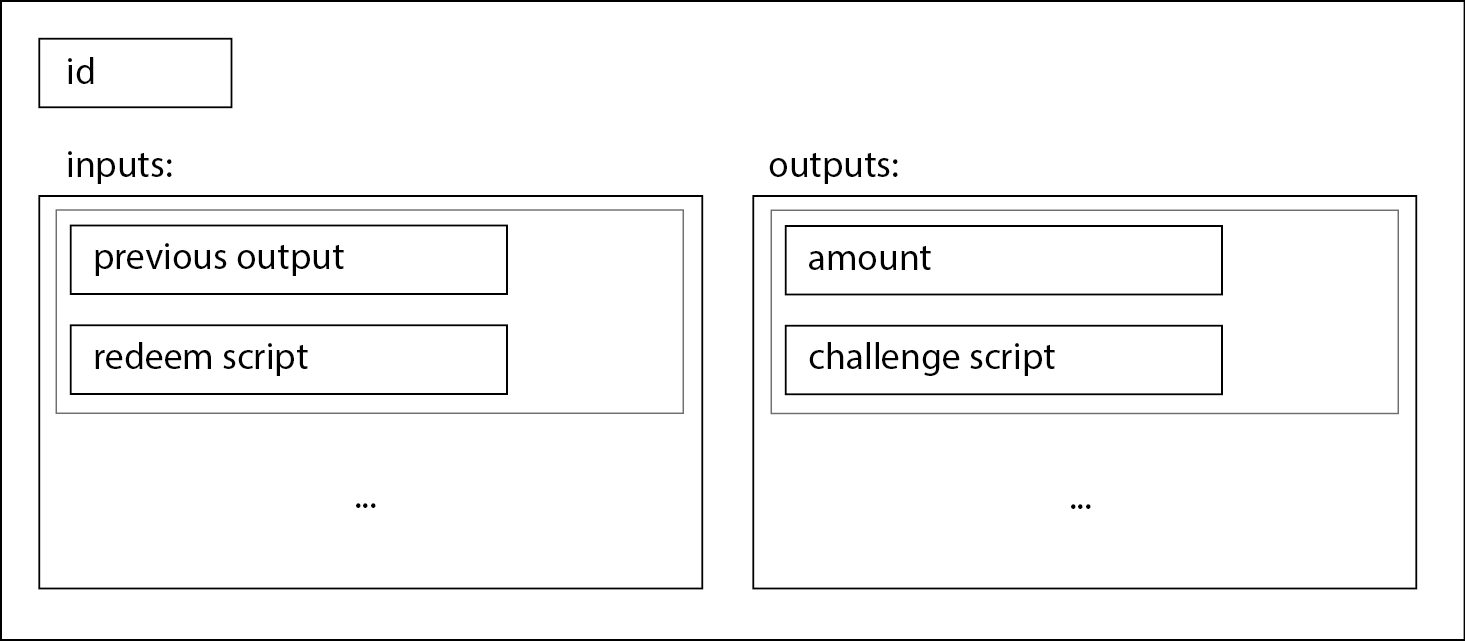
\includegraphics[width=\linewidth]{BitcoinTransaction}
    \caption{Simplified structure of a Bitcoin transaction}
    \label{fig:tx}
  \end{figure}

  \subsection{Thin clients and simplified payment verification}
  \label{subsec:spv}

  Thin clients make use of a scheme called simplified payment verification (SPV). A method which was already described in \cite{nakamoto2008bitcoin}. Thin clients do not have to store the entire blockchain but only block headers with a fixed size of 80 bytes. Thus, thin clients have to rely on full nodes to retrieve relevant transactions. A thin client can verify that a transaction is part of a particular block inside the blockchain. Therefore, it is able to base the trust in the transaction on the depth of the particular block inside the blockchain. 

\section{Capabilities of blockchain-enabled economic objects}
\label{economicObjects}

\subsection{Offer service for payment}

\subsubsection{Description} Assigning a blockchain address to a smart object enables it to receive payments nominated in the native token of the particular blockchain. This allows a smart object to provide services triggered by payments.

\subsubsection{Implementation on Bitcoin blockchain}
\label{subsubsec:offerserviceimp}

As described in section \ref{subsec:signatures} a Bitcoin account is represented essentially as an ECDSA key pair. Thus, Bitcoin accounts can be created ad-hoc in any number. Therefore, a key pair can be generated per offered service. The smart object can either generate key pairs itself or a public key (or Bitcoin address) can be associated with the smart object. In the latter case the private key needs not to be stored on the smart object itself. In order to be aware of a payment the smart object is running a thin client in simplified payment verification mode.

The inherent nature of a distributed consensus system leads to some undesirable properties. A blockchain is more like a settlement system than a payment network. In the best case, it takes on average 10 min until a transaction is included into the Bitcoin blockchain. Thus either the smart objects accepts a transaction that is on the network but not already in the blockchain, and risks fraud by double-spending or it waits until the transaction is included into the blockchain which is inconvenient for the service requester. Furthermore, transactions require a fee which may depend on the load of the network as well as on the size (in bytes). It can be assumed, and will be discussed in the applications section, that in many cases payments will be very small. However, especially in the case of automated machine-to-machine payments transaction sizes of millicents would be desirable.   

There are various proposals of systems which interact with the Bitcoin network but keep a lot of transactions off the network to provide instant nanopayments\footnote{We prefer the term nanopayments over micropayments since micropayments are traditionally on the order of \$1.}. On the one hand there are completely centralized solutions which allow users to send instant transactions without fees between each other \cite{coinbase2015,changetip2015}. However users hand over all control of their bitcoins to those providers. Moreover, current provides focus on human users and are not suitable to handle payments on behalf of smart objects. On the other hand there are solutions which leverage the scripting language to provide trust-minimizing solutions. The basis of all these proposals is the capability to move funds to a shared account. Thus, not one party alone is able to control the funds, but both parties are able to negotiate privately how these funds will be resolved eventually. In Bitcoin this is implemented by multi-signature transactions. A basic mechanism that underlies most of the systems and proposals is the payment channel mechanism \cite{channels2015}. After establishing a payment channel between two parties, which involves the set up of a private refund transaction and a published 2-of-2 multi-signature transaction, the payee can accept transactions, spending the funds, immediately. The basic payment channel is one way and needs to be established between every pair of peers that like to transact. To overcome these limitations payment networks with routing capabilities have been proposed \cite{poonbitcoin,decker2015Duplex}, as well as probabilistic payments schemes \cite{passm2015icropayments}, and schemes based on promissory notes \cite{strawpay}. Payment networks are the most general approach but their implementation is complex and is in need of changes to the Bitcoin protocol mainly due to the malleability issue of Bitcoin transactions \cite{malleability2015}.

\subsubsection{Applications}
Smart objects could offer various services for payment. Especially their ability to interact with the physical world is valuable. In many cases smart objects are augmented by sensors to digitize the physical world. Thus, a smart object may offer its sensing capabilities or measurement data as a service for payment \cite{DBLP:journals/corr/NoyenVWF14,Worner:2014:YSE:2638728.2638786}.

\subsection{Autonomous payment}

\begin{figure*}[!t]
\centering
\subfloat[Macroscopic on-chain payment]{\includegraphics[width=2.5in]{payment}%
\label{fig:payment}}
\hfil
\subfloat[Off-chain nanopayment]{\includegraphics[width=2.5in]{micropayment}%
\label{fig_second_case}}
\caption{Payment and service delivery between smart objects with a payment channel. After setting up a channel. Bitcoin Transactions can be exchanged between peers directly, and payments can be accepted instantly without risk of double spending. In case of a payment channel network the payment might be routed through intermediaries.}
\label{fig:paymentchannel}
\end{figure*}

\subsubsection{Description}

Smart objects that are in possession of private keys controlling blockchain tokens are able to pay for services without any human involvement.

\subsubsection{Implementation on Bitcoin blockchain}

Everything that is needed to perform autonomous payments can be achieved by running a thin client. The smart object needs to be able to generate ECDSA key pairs and to store the private keys securely. It needs to be aware of unspent transactions outputs which it is able to spend. Therefore, it needs to know the state of the blockchain. Furthermore, it needs to create and publish transactions which involves creating signatures.

However, as discussed in section \ref{subsubsec:offerserviceimp}, we assume that payments will be small in most cases and thus payment channels and routed payment networks will have to be used. 

\subsubsection{Applications}

An interesting application is the ad-hoc payment for Internet access on a pay-as-you-go basis. An implementation is described in \cite{siby2013paying}. In this way, a smart object could pay passing smart phones or other closely-located access points for Internet access.  This is in particular interesting for smart city scenarios. There is a recent trend towards Low Power Wide Area Networks (LoRaWAN) which allow cost-efficient connectivity through unregulated frequency bands. However, while low bandwidth (around 1kb/s) is enough for most tasks, over-the-air firmware updates for example can become impossible. 

A further application is outsourcing of computational work. Today, smart objects are outsourcing their computational work to backend infrastructure. However, this backend infrastructure has to be available over the lifetime of the product, and there might be significant round trip times. Thus, in many cases an ad-hoc outsourcing of computational work to devices in physical proximity is advantageous. 
There has been work recently to design fair protocols for multi-party computations \cite{andrychowicz2014secure,bentov2014use,andrychowicz2014fair} and verifiable computations \cite{kumaresan2014use} using Bitcoin that allow the ad-hoc sharing of computational work between untrusted parties. 


\subsection{Transfer of ownership}
\label{subsec:tow}

\subsubsection{Description}

The basic idea is to represent a smart object as a non-fungible token on a blockchain such that it can be transferred between addresses. The smart object has to be controllable by the private key belonging to the respective address. In this way the ownership of a smart property can be transferred publicly and provably between identities on a blockchain. Thereby it is possible to represent permanent transfers of ownership, i.e. selling a smart object, as well as temporary transfer of ownership, i.e. renting a smart object. 


\subsubsection{Implementation on Bitcoin blockchain}

The main technique to represent and track assets besides bitcoin on the Bitcoin blockchain is known as \textit{colored coins}\footnote{https://en.bitcoin.it/wiki/Colored\_Coins}. The intuition behind this term is to taint particular coins, i.e. transaction outputs, in order to associate them with an asset. Typical implementations of this idea are based on OP\_RETURN output scripts. This operator allows to add 40 bytes of metadata to a Bitcoin transaction. Bitcoin nodes neglect everything after an OP\_RETURN operator and the script executes to false. OP\_RETURN outputs are therefore provably undependable, and rules for colored coins are not enforced by Bitcoin nodes. Thus, the simplified payment verification scheme of thin clients is not applicable to these colored coin implementations. 

Since a smart object is able to interact with the blockchain directly we suggest an interactive approach using multi-signature transactions. In this way we can preserve the thin client capabilities. Bitcoin allows to specify output scripts that require $n$ of $m$ signatures to spend the output. In the following scheme we will make use of 2-of-2 and 3-of-3 signatures. 

We define the ownership of a smart object $SO$ to be represented by a multi-signature output with the following script

\begin{lstlisting}[breaklines=true]
OP_2 <pubKeyAlice> <pubKeySO> OP_2 OP_CHECKMULTISIGVERIFY
\end{lstlisting}

$SO$ will recognize Alice as its owner by accepting commands signed with the private key belonging to $pubKeyAlice$. $SO$ will always sign transactions that are signed by its owner.

In order to transfer the ownership from Alice to Bob, Alice will create and sign a transaction that spends the former output to create the new output 

\begin{lstlisting}[breaklines=true]
OP_2 <pubKeyBob> <pubKeySO> OP_2 OP_CHECKMULTISIGVERIFY
\end{lstlisting}

Alice sends the transaction to $SO$ which signs it as well and broadcasts the transaction to the network. As soon as the transaction is in the blockchain with sufficient confirmations $SO$ will recognize Bob as its new owner. The value of an output can also be divided which enables to define multiple owners. Fine grained access control could be implemented either by attaching metadata (using OP\_RETURN) or by  defining key pairs for each level of access rights. 

In a similar way it is possible to transfer the ownership only temporarily out a smart object. For that we are using the timelock feature of Bitcoin transactions. This is a special field in a Bitcoin transaction which allows to specify a timestamp or block number after which a transaction becomes valid. Transaction with a timelock thus can only be added to the blockchain after some point in time. If Alice wants to rent $SO$ to Bob for some time she prepares two transactions: (1) an ownership transaction and (2) a reclaiming transaction. The output script of the ownership transaction is given by

\begin{lstlisting}[breaklines=true]
OP_3 <pubKeyAlice> <pubKeyBob> <pubKeySO> OP_3 OP_CHECKMULTISIGVERIFY
\end{lstlisting}

$SO$ will recognize only Bob as its owner. The reclaiming transaction can spend this output but will be locked until the end of the renting period $T$. Noteworthy, the reclaiming transaction has to be signed by Bob before the ownership transaction is published to the blockchain. Otherwise, Bob might refuse signing and $SO$ will stay under his control. The procedure is illustrated in figure \ref{fig:rent}.

  \begin{figure}[!t]
    \centering
    \includegraphics[width=\columnwidth]{rent}
    \caption{Temporary transfer of ownership of a smart object via the Bitcoin blockchain.}
    \label{fig:rent}
  \end{figure}

Having represented the ownership of a smart object on the blockchain it is possible to sell the smart object for bitcoins as an atomic process. This means, that either the transfer of ownership and the payment are successful or both fail. Thus, the participants of a trade need not to trust each other. 

One way to achieve this is by having the transfer of ownership and the payment within a single transaction. Therefore, Bob prepares a transaction that transfers the ownership of $SO$ from Alice to him and transfers $b$ BTC to an address Alice controls. Bob then partially signs the payment input and sends the transaction to Alice. Alice can accept the offer by signing the ownership transfer input and relaying the transaction to $SO$ which will provide its signature and publish the transaction to the Bitcoin network. The process is illustrated in figure \ref{fig:sale}.


  \begin{figure}[!t]
    \centering
    \includegraphics[width=\columnwidth]{sale}
    \caption{Atomic trade of a smart object via the Bitcoin blockchain.}
    \label{fig:sale}
  \end{figure}


\subsubsection{Applications}

The presented concept of ownership and access management has the advantage of being independent of backend infrastructure. From the perspective of a smart object manufacturer 
the natural application is for commoditized smart objects with a rather long lifetime. Today, providers of connected devices or smart objects have to offer backend infrastructure to manage and configure smart objects. These services have to be provided over the lifetime of a smart object and cause running costs. An interesting application could be Internet-enabled Bluetooth beacons which are distributed in cities worldwide and rented out for marketing campaigns. 


\subsection{Embedded Mining}

\subsubsection{Description}
Proof of work is the main mechanism to reach consensus over the state of the blockchain while providing security against Sybil attacks \cite{douceur2002sybil}. Miners have to solve a computational puzzle based on the current blockchain state in order to extend the blockchain. The winner of this contest can claim newly minted cryptocurrency tokens as well as the transaction fees of the transactions he incorporated into the block. Most cryptocurrencies make use of a proof of work scheme based on Hashcash \cite{back2002hashcash} which consists of the repeating activity of computing SHA-252 hashes. This process can be parallelized and performed by specialized hardware. Hence, the mining process allows a connected device to convert electricity into freshly-minted cryptocurrency tokens.

\subsubsection{Implementation on Bitcoin blockchain}

Bitcoin mining has gone a long way from hobbyists mining on their home computers to data centers filled with specialized mining hardware and access to cheap electricity \cite{taylor2013bitcoin}. In September 2016 the total hash rate of the Bitcoin network is around 450 Petahashes/s. Mining is a probabilistic process with an average rate of return given by 
\begin{equation}
R = \frac{h}{H}V
\end{equation}
where $h$ is the miner's hashing rate, $H$ is the global hashing rate of all Bitcoin miners, and $V$ is the average rate of reward. 
Block generation is a Poisson process which is adjusted every 2000 blocks such that the block generation rate is one every 10 min on average. This is achieved by adjusting the difficulty of the cryptographic puzzle. Every new block allows the miner to claim a block reward. The block reward is modeled as a geometric function which halves approximately every 2 years. Currently the block reward is 25 bitcoins. Hence, $V$ = 25 bitcoins / 10 min. However, since for smart object we will have $\frac{h}{H} \ll 1$ the chance of ever finding a block is negligibly small. After describing the puzzle in more detail we will see why embedded mining is possible nevertheless.

The cryptographic puzzle has two important properties: (1) the solution can be easily and efficiently verified, and (2) the difficulty is adjustable. The puzzle is algorithmically very simple and is implemented in the basic bitcoin core mining software as follows\footnote{https://github.com/bitcoin/bitcoin/blob/master/src/miner.cpp}
\begin{lstlisting}[breaklines=true]
while (1)
  HDR[kNoncePos]++;
  IF (SHA256(SHA256(HDR)) < (65535 << 208)/ DIFFICULTY)
  return; 
\end{lstlisting}
Basically the hash of the block header, which entails a random value called a nonce, has to be smaller than a predefined number. A miner has to vary the nonce until this condition is met\footnote{Since the nonce is only a 32 bit integer it is necessary to change other fields of the block header as well. The most obvious field is the time. Another trick used in the Stratum mining protocol \cite{stratum} is to change the merkle root by adapting the coinbase transaction.}. Since iterations are independent of each other the hashing process can be parallelized and distributed. Furthermore, the SHA-252 algorithm can be implemented directly as a application-specific integrated circuit (ASIC). This means the ability to hash very efficiently could readily be integrated into systems-on-chip (SoC) for smart objects\footnote{See \cite{mack2015multiple} for a discussion of the trend towards integration termed as Moore's Law 3.0}. Therefore, having billions of connected devices of which a significant subset is coordinated to hash collaboratively will have the ability to find blocks and to generate bitcoins.

%\subsubsection{Applications}
%???  

\section{Discussion}

\subsection{Hardware requirements}

\subsubsection*{Computation}
Cryptographic operations like signing and verifying signatures are computationally expensive on CPUs in small embedded devices. However, these operations can also be executed by dedicated hardware (e.g. ASICs).  

\subsubsection*{Storage}
As discussed in section \ref{subsec:spv} thin clients only store block headers. A block header in Bitcoin is 80 bytes. Today (September 2015), this leads to storage requirements of about 30 MB with a constant growth rate of about 4.2 MB/year.

\subsubsection*{Communication}
In order to keep communication requirements low it is advisable to factory-preload the block headers. Otherwise the initial syncing process would be prohibitive in low-bandwidth scenarios. In addition to block headers, transactions for SPV proofs have to be downloaded. An average transaction has around 600 bytes and today a block consists of about 1000 transactions. This means for an SPV proof that a transaction is in a particular block approximately 600 bytes * $\log_2(1000)$ = 6 kb have to be transfered.

%\subsubsection*{Security}


\subsection{Transaction fees}
Maintaining a proof of work based blockchain is expensive, and costs are proportional to the security. Thus, transactions that need to be included in the blockchain may have to include fees in order to be considered by miners. In principle every miner can follow his own rules concerning fees. However, the reference implementation of the Bitcoin client calculates fees according to the age of the outputs that are spent, their value, and the size of the transaction. Today, the typical transaction fee is 0.0001 bitcoin which corresponds to 2.3 cents. Noteworthy, transaction fees currently constitute only 0.5 - 1\% of the block reward. Furthermore, Bitcoin has a maximum block size of 1 MB which is subject to heavy debate \cite{blocksize}. If Bitcoin adoption continues to rise space in blocks will get scarce and transactions will have to provide higher fees in order to be considered by miners. 

\subsection{Extending Bitcoin for non-currency applications}
Bitcoin was designed to provide a peer-to-peer electronic cash system. The open and permissionless nature is an ideal foundation to build machine-to-machine payments upon. We've seen in section \ref{subsec:tow} that we can also represent device ownership with Bitcoin. However if we wanted to store fine-grained access rights or describe complex contractual terms the Bitcoin transaction data structure and its restricted scripting language becomes prohibitive and fees may be of concern. There are basically three design choices that can be pursued to circumvent these problems.

\subsubsection*{Altcoin and altchains}
Bitcoin is open source and thus one can easily fork the codebase and adapt it to meet application specific needs. Forks which aim to be alternative cryptocurrencies are termed altcoins. Forks which provide non-currency applications based on a blockchain are termed altchains. One of the first altchains that was released is Namecoin \cite{namecoin} which provides an information registration and transfer system by allowing to store name/value pairs on its blockchain. Therefore, it could be utilized as an updateable device and service registry. However, the issue with altcoins is security. Either an Bitcoin-incompatible proof of work mechanism is used which is vulnerable to botnet attacks or it has to be merge-mined with Bitcoin. Namecoin for example follows the latter path but is thus vulnerable to attacks of large Bitcoin mining pools. Ethereum on the other hand follows the former path but uses a proof of work scheme that is GPU-friendly instead of CPU-friendly or ASIC-friendly in the hope to minimize the risk of botnet attacks. In general every altcoin or altchain has to provide a blockchain-native token in order to incentive participation.

\subsubsection*{Sidechains}

An alternative to the multi-currency scenario described above is enabled by sidechains \cite{back2014enabling}. Sidechains are blockchains that are connected to a main blockchain by a two-way peg mechanism which allows to transfer assets between blockchains. In principle sidechains have the same security issues as altcoins, but don't have to introduce new currencies

\subsubsection*{Mixed systems}

Today's blockchain technology involves a full node to store an entire copy of the blockchain and to do every computation in order to have a consensus of the current state of the system. Thus, it is very expensive to run complex computations or to store data on a blockchain. Analogous to payment networks, which keep most of the payment transactions except setup and settlement transaction off-blockchain, data storage and computation can be done off-blockchain in a way that is controllable and auditable via the blockchain.

\section{Non-academic approaches towards economic objects}

In contrast to academia which hasn't taken interest in the toolkit provided by cryptocurrencies and blockchain technology to address issues concerning the Internet of Things, work has been done by industry and start up companies.  

The IBM Institute for Business Value has proposed the Autonomous Decentralized Peer-To-Peer Telemetry (ADEPT) platform  \cite{brody2014device,pureswaran2015empowering} which is based on BitTorrent \cite{cohen2008bittorrent}, Telehash \cite{Telehash} and a private fork of Ethereum \cite{buterin2014ethereum}. Thereby, an Ethereum-based blockchain is used as a device registry and to enforce device coordination.

Filament is working on the open Distributed Sensor Transactions (DIST) platform \cite{filament}. The platform aims to make use of the Bitcoin blockchain to provide a device registry, ownership verification and payments. Thus, it will provide implementations of the main concepts presented in this paper. Details concerning the micropayment implementation can be found in \cite{pennybank}.

21, a silicon valley-based start up company with profound venture capital investments and partnerships with chip manufacturers, \cite{21,21medium} aims to make bitcoin a resource of every connected device by providing embedded mining chips, and development tools to make API endpoints accessible in exchange for Bitcoin nanopayments. At time of writing the product is only available for pre-order and no details concerning the underlying technology is available. 

%\section{Open research questions}
\section{Research perspectives}
As discussed in section \ref{subsubsec:offerserviceimp} a main building block for economic objects are nanopayment technologies. The most promising approaches  

\section{Conclusion}



% An example of a floating figure using the graphicx package.
% Note that \label must occur AFTER (or within) \caption.
% For figures, \caption should occur after the \includegraphics.
% Note that IEEEtran v1.7 and later has special internal code that
% is designed to preserve the operation of \label within \caption
% even when the captionsoff option is in effect. However, because
% of issues like this, it may be the safest practice to put all your
% \label just after \caption rather than within \caption{}.
%
% Reminder: the "draftcls" or "draftclsnofoot", not "draft", class
% option should be used if it is desired that the figures are to be
% displayed while in draft mode.
%
%\begin{figure}[!t]
%\centering
%\includegraphics[width=2.5in]{myfigure}
% where an .eps filename suffix will be assumed under latex, 
% and a .pdf suffix will be assumed for pdflatex; or what has been declared
% via \DeclareGraphicsExtensions.
%\caption{Simulation results for the network.}
%\label{fig_sim}
%\end{figure}

% Note that IEEE typically puts floats only at the top, even when this
% results in a large percentage of a column being occupied by floats.


% An example of a double column floating figure using two subfigures.
% (The subfig.sty package must be loaded for this to work.)
% The subfigure \label commands are set within each subfloat command,
% and the \label for the overall figure must come after \caption.
% \hfil is used as a separator to get equal spacing.
% Watch out that the combined width of all the subfigures on a 
% line do not exceed the text width or a line break will occur.
%
%\begin{figure*}[!t]
%\centering
%\subfloat[Case I]{\includegraphics[width=2.5in]{box}%
%\label{fig_first_case}}
%\hfil
%\subfloat[Case II]{\includegraphics[width=2.5in]{box}%
%\label{fig_second_case}}
%\caption{Simulation results for the network.}
%\label{fig_sim}
%\end{figure*}
%
% Note that often IEEE papers with subfigures do not employ subfigure
% captions (using the optional argument to \subfloat[]), but instead will
% reference/describe all of them (a), (b), etc., within the main caption.
% Be aware that for subfig.sty to generate the (a), (b), etc., subfigure
% labels, the optional argument to \subfloat must be present. If a
% subcaption is not desired, just leave its contents blank,
% e.g., \subfloat[].


% An example of a floating table. Note that, for IEEE style tables, the
% \caption command should come BEFORE the table and, given that table
% captions serve much like titles, are usually capitalized except for words
% such as a, an, and, as, at, but, by, for, in, nor, of, on, or, the, to
% and up, which are usually not capitalized unless they are the first or
% last word of the caption. Table text will default to \footnotesize as
% IEEE normally uses this smaller font for tables.
% The \label must come after \caption as always.
%
%\begin{table}[!t]
%% increase table row spacing, adjust to taste
%\renewcommand{\arraystretch}{1.3}
% if using array.sty, it might be a good idea to tweak the value of
% \extrarowheight as needed to properly center the text within the cells
%\caption{An Example of a Table}
%\label{table_example}
%\centering
%% Some packages, such as MDW tools, offer better commands for making tables
%% than the plain LaTeX2e tabular which is used here.
%\begin{tabular}{|c||c|}
%\hline
%One & Two\\
%\hline
%Three & Four\\
%\hline
%\end{tabular}
%\end{table}


% Note that the IEEE does not put floats in the very first column
% - or typically anywhere on the first page for that matter. Also,
% in-text middle ("here") positioning is typically not used, but it
% is allowed and encouraged for Computer Society conferences (but
% not Computer Society journals). Most IEEE journals/conferences use
% top floats exclusively. 
% Note that, LaTeX2e, unlike IEEE journals/conferences, places
% footnotes above bottom floats. This can be corrected via the
% \fnbelowfloat command of the stfloats package.



% conference papers do not normally have an appendix



% use section* for acknowledgment
\ifCLASSOPTIONcompsoc
  % The Computer Society usually uses the plural form
  \section*{Acknowledgments}
\else
  % regular IEEE prefers the singular form
  \section*{Acknowledgment}
\fi


Blank for review





% trigger a \newpage just before the given reference
% number - used to balance the columns on the last page
% adjust value as needed - may need to be readjusted if
% the document is modified later
%\IEEEtriggeratref{8}
% The "triggered" command can be changed if desired:
%\IEEEtriggercmd{\enlargethispage{-5in}}

% references section

% can use a bibliography generated by BibTeX as a .bbl file
% BibTeX documentation can be easily obtained at:
% http://www.ctan.org/tex-archive/biblio/bibtex/contrib/doc/
% The IEEEtran BibTeX style support page is at:
% http://www.michaelshell.org/tex/ieeetran/bibtex/
\bibliographystyle{IEEEtran}
% argument is your BibTeX string definitions and bibliography database(s)
\bibliography{percom}
%
% <OR> manually copy in the resultant .bbl file
% set second argument of \begin to the number of references
% (used to reserve space for the reference number labels box)





% that's all folks
\end{document}


